\section{Revisão Bibliográfica} \label{secao:rev_bib}

A linguagem de programação Java foi escolhida para a criação da ferramenta, os motivos para essa escolha foram:

\newcommand{\JVM}{\sigla{JVM}{Java Virtual Machine}}

\begin{itemize}
    \item Multiplataforma: Java é uma linguagem capaz de ser executada em qualquer sistema que possua uma \JVM, sua execução e desenvolvimento independe do sistema, permitindo que a aplicação desenvolvida não sofra essa restrição.
    \item Desempenho: entre as linguagens de programação que são interpretadas, Java possui um desempenho melhor por ser compilada e interpretada, gerando um código intermediário que é executado pela \JVM.
    \item Facilidade e didática: Java é uma linguagem que permite certas comodidades ao programador com um bom balanço de desempenho, como a ferramenta desenvolvida foi utilizada para estudos e é de uso genérico, as facilidades fornecidas pela linguagem são importante para agilizar e pela validação do trabalho.
    \item Modelagem: a modelagem de classes fornecida por Java ajudam no entendimento e no reuso da biblioteca desenvolvida.
\end{itemize}

Nesse projeto há uma contextualização do problema nos seguintes moldes:

\begin{itemize}
    \item Indivíduo: um indivíduo é a representação de um jogador que possui uma pontuação provida da função \fitness de acordo com as respostas produzidas por esse jogador.
    \item Gene: um gene é uma entidade capaz de provocar uma resposta. Para cada tipo de respostas há um grupo de genes.
    \item Disputa: é uma função entre dois indivíduos que gera um vencedor e um perdedor com base na função \fitness. Uma disputa deve necessariamente retornar o quão melhor um indivíduo foi em relação a outro.
\end{itemize}

Por tanto, o indivíduo que possui os melhores genes terá uma função \fitness melhor e ganhará mais disputas.

A inspiração do paradigma da Computação Evolutiva vem da evolução natural formalizada por Darwin\footnote
{Ridley , M. (1996). Evolution. Blackwell Science.}.
Algoritmos que embebidos desta teste possuem passos genéricos capazes de resolver um grande número de problemas práticos, e possuem caractéristicas como auto-organização e comportamento adaptativo\footnote
{Goldberg, D. E. and Holland, J. H. (1988). Genetic Algorithms and Machine Learning: Introduction to the Special Issue on Genetic Algorithms. Machine Learning.},
portanto são capazes de tratar problemas computacionalmente complexos com uma ferramenta de propósito geral. Por outro lado, esses algoritmos não garantem a obtenção de uma solução ótima\footnote
{Zuben, F . J. V . (2000). Computação evolutiva: Uma abordagem pragmática. Anais da 1ª Jornada de Estudos em Computação de Piracicaba e região (1ª JECOMP), 1:25-45.}
por poder convergir para soluções localmente ótimas.

\section{Algoritmos evolutivos}
Os algoritmos evolutivos podem ser resumidos em um roteiro básico de procedimentos\footnote
{Todd, P. M. e Miller, G. F., (1997) Biodiversity Through Sexual Selection. In Artificial Life V, Langton, C. G. and Shimohara, K. (Eds.), Publisher: MIT Press, Cambridge, MA. USA, pp. 289-299.}
que são adaptados de acordo com o contexto do problema a ser solucionado\footnote
{Werger, B. B. e Mataric, M. J. (1999) Exploiting Embodiment in Multi-Robot Teams. Report ID: Technical Report IRIS-99-378, University of Southern California, Institute for Robotics and Intelligent Systems, 14p}\footnote
{Mitchell, M. (1995) Genetic Algorithms and Artificial Life. In Artificial Life An Overview, Langton, C. G. (Ed.), Publisher: MIT Press, pp. 267-289.}.
Um algoritmo evolutivo é usualmente composto por:

\newcommand{\crossover}{\textit{crossover}\xspace}

\begin{itemize}
    \item Representação de genes dos indivíduos: Biologicamente, cada gene representa uma característica do indivíduo, e o cromossomo, que é o conjunto de genes de um indivíduo, representa uma o indivíduo. Computacionalmente, o cromossomo representa um candidato à solução do problema e o gene representa uma função para obtenção de uma resposta.
    \item Função \fitness (ou de adaptação): indica, para cada indivíduo, o valor de aptidão, mostrando a aproximação da solução proposta pelo indivíduo em relação à solução procurada.
    \item Função de reprodução: Determina novos indivíduos que representarão a próxima geração da população do algoritmo herdando características positivas que são encontradas nos indivíduos com uma maior função \fitness (ou mais aptos), propagando seus genes. O \crossover e mutações ocorrem na função de reprodução, de modo análogo ao biológico.
\end{itemize}

Em um algoritmo evolutivo, a população inicial é constituída por indivíduos com genes aleatórios, ou seja, o início do algoritmo parte de uma solução aleatória e a cada geração, o valor de \fitness ou adequação é calculado em cada indivíduo. A função de reprodução gera novos indivíduos e as características positivas de cada indivíduo pode ser propagada para a nova geração, assim a solução caminha para uma resposta adequada. O fluxograma na Figura \ref{figura:fluxograma_ae} representa estas etapas.

\begin{figure}[htb]
    \caption{Fluxograma de uma implementação típica de um algoritmo evolutivo.}
    \label{figura:fluxograma_ae}
    \centering
    %scale=0.8
    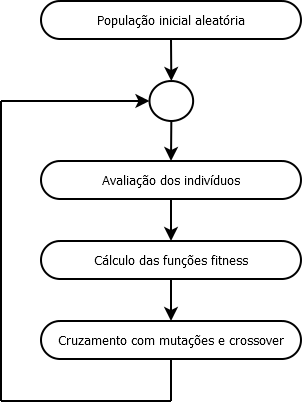
\includegraphics[scale=1]{images/dia/fluxograma-ae}
    \fautor
\end{figure}